\documentclass[10pt]{article}
\usepackage[T1]{fontenc}
\usepackage[utf8]{inputenc}
% \usepackage{lmodern}
%\usepackage[adobe-utopia,uppercase=upright,greeklowercase=upright]{mathdesign}
\usepackage[adobe-utopia]{mathdesign}
%\usepackage{minionpro}
% \usepackage{pifont}
% \usepackage{amssymb}
\usepackage{amsmath}
\usepackage[francais]{babel}
% \usepackage[francais]{varioref}
\usepackage[dvips]{graphicx}

\usepackage{framed}
\usepackage[normalem]{ulem}
\usepackage{fancyhdr}
\usepackage{titlesec}
\usepackage{vmargin}
\usepackage{longtable}

\usepackage{ifthen}


%\usepackage{epsfig}
\usepackage{subfig}

\usepackage{multirow}
\usepackage{multicol} % Portions de texte en colonnes
\usepackage{flafter}%floatants après la référence



\usepackage{color}
\usepackage{colortbl}


\definecolor{gris25}{gray}{0.75}
\definecolor{bleu}{RGB}{18,33,98}
\definecolor{bleuf}{RGB}{42,94,171}
\definecolor{bleuc}{RGB}{231,239,247}
\definecolor{rougef}{RGB}{185,18,27}
\definecolor{rougec}{RGB}{255,230,231}
\definecolor{vertf}{RGB}{103,126,82}
\definecolor{vertc}{RGB}{220,255,191}

\newenvironment{rem}[1][\hsize]%
{%
    \def\FrameCommand
    {%
\rotatebox{90}{\textit{\textsf{Remarque}}} 
        {\color{bleuf}\vrule width 3pt}%
        \hspace{0pt}%must no space.
        \fboxsep=\FrameSep\colorbox{bleuc}%
    }%
    \MakeFramed{\hsize#1\advance\hsize-\width\FrameRestore}%
}%
{\endMakeFramed}%


\newenvironment{contexte}[1][\hsize]%
{%
    \def\FrameCommand
    {%
\rotatebox{90}{\textit{\textsf{Contexte}}} 
        {\color{bleuf}\vrule width 3pt}%
        \hspace{0pt}%must no space.
        \fboxsep=\FrameSep\colorbox{bleuc}%
    }%
    \MakeFramed{\hsize#1\advance\hsize-\width\FrameRestore}%
}%
{\endMakeFramed}%

\newenvironment{savoir}[1][\hsize]%
{%
    \def\FrameCommand
    {%
\rotatebox{90}{\textit{\textsf{Savoir}}} 
        {\color{bleuf}\vrule width 3pt}%
        \hspace{0pt}%must no space.
        \fboxsep=\FrameSep\colorbox{bleuc}%
    }%
    \MakeFramed{\hsize#1\advance\hsize-\width\FrameRestore}%
}%
{\endMakeFramed}%

\newenvironment{prob}[1][\hsize]%
{%
    \def\FrameCommand%
    {%
\rotatebox{90}{\textit{\textsf{ Problématique}}} 
        {\color{rougef}\vrule width 3pt}%
        \hspace{0pt}%must no space.
        \fboxsep=\FrameSep\colorbox{rougec}%
    }%
    \MakeFramed{\hsize#1\advance\hsize-\width\FrameRestore}%
}%
{\endMakeFramed}%

\newenvironment{obj}[1][\hsize]%
{%
    \def\FrameCommand%
    {%
\rotatebox{90}{\textit{\textsf{ $\;$}}} 
        {\color{rougef}\vrule width 3pt}%
        \hspace{0pt}%must no space.
        \fboxsep=\FrameSep\colorbox{rougec}%
    }%
    \MakeFramed{\hsize#1\advance\hsize-\width\FrameRestore}%
}%
{\endMakeFramed}%

\newenvironment{defi}[1][\hsize]%
{%
    \def\FrameCommand%
    {%
\rotatebox{90}{\textit{\textsf{Définition\\}}} 
        {\color{bleuf}\vrule width 3pt}%
        \hspace{0pt}%must no space.
        \fboxsep=\FrameSep\colorbox{bleuc}%
    }%
    \MakeFramed{\hsize#1\advance\hsize-\width\FrameRestore}%
}%
{\endMakeFramed}%


\newenvironment{hypo}[1][\hsize]%
{%
    \def\FrameCommand%
    {%
\rotatebox{90}{\textit{\textsf{Hypothèse\\}}} 
        {\color{bleuf}\vrule width 3pt}%
        \hspace{0pt}%must no space.
        \fboxsep=\FrameSep\colorbox{bleuc}%
    }%
    \MakeFramed{\hsize#1\advance\hsize-\width\FrameRestore}%
}%
{\endMakeFramed}%


\newenvironment{prop}[1][\hsize]%
{%
    \def\FrameCommand%
    {%
\rotatebox{90}{\textit{\textsf{Propriété\\}}} 
        {\color{bleuf}\vrule width 3pt}%
        \hspace{0pt}%must no space.
        \fboxsep=\FrameSep\colorbox{bleuc}%
    }%
    \MakeFramed{\hsize#1\advance\hsize-\width\FrameRestore}%
}%
{\endMakeFramed}%

\newenvironment{props}[1][\hsize]%
{%
    \def\FrameCommand%
    {%
\rotatebox{90}{\textit{\textsf{Propriétés\\}}} 
        {\color{bleuf}\vrule width 3pt}%
        \hspace{0pt}%must no space.
        \fboxsep=\FrameSep\colorbox{bleuc}%
    }%
    \MakeFramed{\hsize#1\advance\hsize-\width\FrameRestore}%
}%
{\endMakeFramed}%

\newenvironment{exemple}[1][\hsize]%
{%
    \def\FrameCommand%
    {%
\rotatebox{90}{\textit{\textsf{Exemple\\}}} 
        {\color{vertf}\vrule width 3pt}%
        \hspace{0pt}%must no space.
        \fboxsep=\FrameSep\colorbox{vertc}%
    }%
    \MakeFramed{\hsize#1\advance\hsize-\width\FrameRestore}%
}%
{\endMakeFramed}%

\newenvironment{resultat}[1][\hsize]%
{%
    \def\FrameCommand%
    {%
\rotatebox{90}{\textit{\textsf{Résultat\\}}} 
        {\color{rougef}\vrule width 3pt}%
        \hspace{0pt}%must no space.
        \fboxsep=\FrameSep\colorbox{rougec}%
    }%
    \MakeFramed{\hsize#1\advance\hsize-\width\FrameRestore}%
}%
{\endMakeFramed}%

\newenvironment{methode}[1][\hsize]%
{%
    \def\FrameCommand%
    {%
\rotatebox{90}{\textit{\textsf{Méthode\\}}} 
        {\color{rougef}\vrule width 3pt}%
        \hspace{0pt}%must no space.
        \fboxsep=\FrameSep\colorbox{rougec}%
    }%
    \MakeFramed{\hsize#1\advance\hsize-\width\FrameRestore}%
}%
{\endMakeFramed}%

\newenvironment{theo}[1][\hsize]%
{%
    \def\FrameCommand%
    {%
\rotatebox{90}{\textit{\textsf{Théorème\\}}} 
        {\color{rougef}\vrule width 3pt}%
        \hspace{0pt}%must no space.
        \fboxsep=\FrameSep\colorbox{rougec}%
    }%
    \MakeFramed{\hsize#1\advance\hsize-\width\FrameRestore}%
}%
{\endMakeFramed}%

\newenvironment{warn}[1][\hsize]%
{%
    \def\FrameCommand%
    {%
\rotatebox{90}{\textit{\textsf{Attention\\}}} 
        {\color{rougef}\vrule width 3pt}%
        \hspace{0pt}%must no space.
        \fboxsep=\FrameSep\colorbox{rougec}%
    }%
    \MakeFramed{\hsize#1\advance\hsize-\width\FrameRestore}%
}%
{\endMakeFramed}%

% \usepackage{pstricks}
%\usepackage{minitoc}
% \setcounter{minitocdepth}{4}

\setcounter{tocdepth}{2}

% \mtcselectlanguage{french} 

%\usepackage{draftcopy}% "Brouillon"
% \usepackage{floatflt}
\usepackage{psfrag}
%\usepackage{listings} % Permet d'insérer du code de programmation
\renewcommand{\baselinestretch}{1.2}

% Changer la numérotation des figures :
% ------------------------------------
% \makeatletter
% \renewcommand{\thefigure}{\ifnum \c@section>\z@ \thesection.\fi
%  \@arabic\c@figure}
% \@addtoreset{figure}{section}
% \makeatother
 


%%%%%%%%%%%%
% Définition des vecteurs %
%%%%%%%%%%%%
 \newcommand{\vect}[1]{\overrightarrow{#1}}

%%%%%%%%%%%%
% Définition des torseusr %
%%%%%%%%%%%%

 \newcommand{\torseur}[1]{%
\left\{{#1}\right\}
}

\newcommand{\torseurcin}[3]{%
\left\{\mathcal{#1} \left(#2/#3 \right) \right\}
}

\newcommand{\torseurstat}[3]{%
\left\{\mathcal{#1} \left(#2\rightarrow #3 \right) \right\}
}

 \newcommand{\torseurc}[8]{%
%\left\{#1 \right\}=
\left\{
{#1}
\right\}
 = 
\left\{%
\begin{array}{cc}%
{#2} & {#5}\\%
{#3} & {#6}\\%
{#4} & {#7}\\%
\end{array}%
\right\}_{#8}%
}

 \newcommand{\torseurcol}[7]{
\left\{%
\begin{array}{cc}%
{#1} & {#4}\\%
{#2} & {#5}\\%
{#3} & {#6}\\%
\end{array}%
\right\}_{#7}%
}

 \newcommand{\torseurl}[3]{%
%\left\{\mathcal{#1}\right\}_{#2}=%
\left\{%
\begin{array}{l}%
{#1} \\%
{#2} %
\end{array}%
\right\}_{#3}%
}

 \newcommand{\vectv}[3]{%
\vect{V\left( {#1} \in {#2}/{#3}\right)}
}


\newcommand{\vectf}[2]{%
\vect{R\left( {#1} \rightarrow {#2}\right)}
}

\newcommand{\vectm}[3]{%
\vect{\mathcal{M}\left( {#1}, {#2} \rightarrow {#3}\right)}
}


 \newcommand{\vectg}[3]{%
\vect{\Gamma \left( {#1} \in {#2}/{#3}\right)}
}

 \newcommand{\vecto}[2]{%
\vect{\Omega\left( {#1}/{#2}\right)}
}
% }$$\left\{\mathcal{#1} \right\}_{#2} =%
% \left\{%
% \begin{array}{c}%
%  #3 \\%
%  #4 %
% \end{array}%
% \right\}_{#5}}

%  ------------------------------------------
% | Modification du formatage des sections : | 
%  ------------------------------------------

% Grands titres :
% ---------------

\newcommand{\titre}[1]{%
\begin{center}
      \bigskip
      \rule{\textwidth}{1pt}
      \par\vspace{0.1cm}
      
      \textbf{\large #1}
      \par\rule{\textwidth}{1pt}
    \end{center}
    \bigskip
  }

% Supprime le numéro du chapitre dans la numérotation des sections:
% -----------------------------------------------------------------
\makeatletter
\renewcommand{\thesection}{\@arabic\c@section}
\makeatother


% \titleformat{\chapter}[display]
% {\normalfont\Large\filcenter}
% {}
% {1pc}
% {\titlerule[1pt]
%   \vspace{1pc}%
%   \Huge}[\vspace{1ex}%
% \titlerule]


%%%% Chapitres Comme PY Pechard %%%%%%%%%
% numéro du chapitre
\DeclareFixedFont{\chapnumfont}{OT1}{phv}{b}{n}{80pt}
% pour le mot « Chapitre »
\DeclareFixedFont{\chapchapfont}{OT1}{phv}{m}{it}{40pt}
% pour le titre
\DeclareFixedFont{\chaptitfont}{T1}{phv}{b}{n}{25pt}

\definecolor{gris}{gray}{0.75}
\titleformat{\chapter}[display]%
	{\sffamily}%
	{\filleft\chapchapfont\color{gris}\chaptertitlename\
	\\
	\vspace{12pt}
	\chapnumfont\thechapter}%
	{16pt}%
	{\filleft\chaptitfont}%
	[\vspace{6pt}\titlerule\titlerule\titlerule]

%%%%  Fin Chapitres Comme PY Pechard %%%%%%%%%


% Section, subsection, subsubsection sans serifs :
% % ----------------------------------------------

% \makeatletter
% \renewcommand{\section}{\@startsection{section}{0}{0mm}%
% {\baselineskip}{.3\baselineskip}%
% {\normalfont\sffamily\Large\textbf}}%
% \makeatother

\makeatletter
\renewcommand{\@seccntformat}[1]{{\textcolor{bleu}{\csname
the#1\endcsname}\hspace{0.5em}}}
\makeatother

\makeatletter
\renewcommand{\section}{\@startsection{section}{1}{\z@}%
                       {-4ex \@plus -1ex \@minus -.4ex}%
                       {1ex \@plus.2ex }%
                       {\normalfont\Large\sffamily\bfseries}}%
\makeatother
 
\makeatletter
\renewcommand{\subsection}{\@startsection {subsection}{2}{\z@}
                          {-3ex \@plus -0.1ex \@minus -.4ex}%
                          {0.5ex \@plus.2ex }%
                          {\normalfont\large\sffamily\bfseries}}
\makeatother
 
\makeatletter
\renewcommand{\subsubsection}{\@startsection {subsubsection}{3}{\z@}
                          {-2ex \@plus -0.1ex \@minus -.2ex}%
                          {0.2ex \@plus.2ex }%
                          {\normalfont\large\sffamily\bfseries}}
\makeatother
 
\makeatletter             
\renewcommand{\paragraph}{\@startsection{paragraph}{4}{\z@}%
                                    {-2ex \@plus-.2ex \@minus .2ex}%
                                    {0.1ex}%               
{\normalfont\sffamily\bfseries}}
\makeatother
 
\makeatletter             
\renewcommand{\paragraph}{\@startsection{paragraph}{4}{\z@}%
                                    {-2ex \@plus-.2ex \@minus .2ex}%
                                    {0.1ex}%               
{\normalfont\sffamily\bfseries Question }}
\makeatother

\renewcommand{\theparagraph}{\arabic{paragraph}} 


\makeatletter
\renewcommand{\subparagraph}{\@startsection{subparagraph}{5}{\z@}%
                                       {-2ex \@plus-.1ex \@minus .2ex}%
                                       {0.1ex}%
				    {\normalfont\normalsize\sffamily\bfseries}}
\makeatletter
% \makeatletter
% \renewcommand{\subsection}{\@startsection{subsection}{1}{2mm}%
% {\baselineskip}{.3\baselineskip}%
% {\normalfont\sffamily\large\textbf}}%
% \makeatother
% 
% \makeatletter
% \renewcommand{\subsubsection}{\@startsection{subsubsection}{2}{4mm}%
% {\baselineskip}{.15\baselineskip}%
% {\normalfont\sffamily\large\textbf}}%
% \makeatother
% 
% \makeatletter
% \renewcommand{\paragraph}{\@startsection{paragraph}{3}{6mm}%
% {\baselineskip}{.15\baselineskip}%
% {\normalfont\sffamily\large\textbf}}%
% \makeatother
 
\setcounter{secnumdepth}{4}


%  --------
% | Marges |
%  --------


% \setmarginsrb{2.5cm}{1.5cm}{2.5cm}{2cm}{1cm}{1cm}{1cm}{1cm}
\setmarginsrb{1.5cm}{1cm}{1cm}{1.5cm}{1cm}{1cm}{1cm}{1cm}

% Changer les marges localement :
% -----------------------------
\newenvironment{changemargin}[2]{\begin{list}{}{%
\setlength{\topsep}{0pt}%
\setlength{\leftmargin}{0pt}%
\setlength{\rightmargin}{0pt}%
\setlength{\listparindent}{\parindent}%
\setlength{\itemindent}{\parindent}%
\setlength{\parsep}{0pt plus 1pt}%
\addtolength{\leftmargin}{#1}%
\addtolength{\rightmargin}{#2}%
}\item }{\end{list}}



\usepackage{pst-solides3d}
\usepackage{titletoc}
\titlecontents{chapter}[+3pc]
  {\addvspace{10pt}\sffamily\bfseries}
{\contentslabel[{\pscirclebox[fillstyle=solid,fillcolor=gray!25,
linecolor=gray!25,framesep=4pt]{\textcolor{white}{\thecontentslabel}}}]{2.5pc}}
  {}
  {\dotfill \normalfont\thecontentspage\ }

\titlecontents{section}[3pc]
  {\addvspace{2pt}\sffamily}
  {\contentslabel[\thecontentslabel]{1.8pc}}
  {}
  {\dotfill \normalfont\thecontentspage\ }

\titlecontents{subsection}[5pc]
  {\addvspace{2pt}\sffamily}
  {\contentslabel[\thecontentslabel]{1.8pc}}
  {}
  {\dotfill \normalfont\thecontentspage\ }

\titlecontents{subsubsection}[8pc]
  {\addvspace{2pt}\sffamily}
  {\contentslabel[\thecontentslabel]{3pc}}
  {}
  {\dotfill \normalfont\thecontentspage\ }
%{\;\titlerule\;\normalfont\thecontentspage\ }

\titlecontents{paragraph}[9pc]
  {\addvspace{2pt}\sffamily}
  {\contentslabel[\thecontentslabel]{3.5pc}}
  {}
  {\dotfill \normalfont\thecontentspage\ }



%\usepackage{algorithm}
%\usepackage{algorithmic}
\usepackage[french]{algorithm2e}

\SetKwBlock{Fonction}{Début Fonction}{Fin Fonction}
\SetKwComment{Comment}{start}{end}
% Python sources

\usepackage{listings}
\lstloadlanguages{R}   % pour regler les pb d accent utf8 dans les codes
\lstset{language=R} % pour regler les pb d accent utf8 dans les codes

\usepackage{textcomp}
\usepackage{setspace}
%\usepackage{palatino}

%\usepackage{color}
\definecolor{Bleu}{rgb}{0.1,0.1,1.0}
\definecolor{Noir}{rgb}{0,0,0}
\definecolor{Grau}{rgb}{0.5,0.5,0.5}
\definecolor{DunkelGrau}{rgb}{0.15,0.15,0.15}
\definecolor{Hellbraun}{rgb}{0.5,0.25,0.0}
\definecolor{Magenta}{rgb}{1.0,0.0,1.0}
\definecolor{Gris}{gray}{0.5}
\definecolor{Vert}{rgb}{0,0.5,0}
\definecolor{SourceHintergrund}{rgb}{1,1.0,0.95}


%
\renewcommand{\lstlistlistingname}{Listings}
\renewcommand{\lstlistingname}{Listing}

\lstnewenvironment{python}[1][]{
\lstset{
%escapeinside={\%*}{*)},
%inputencoding=utf8,   % pour regler les pb d accent utf8 dans les codes
%extendedchars=true,   % pour regler les pb d accent utf8 dans les codes
language=python,
basicstyle=\sffamily\footnotesize, 	
stringstyle=\color{red}, 
showstringspaces=false, 
alsoletter={1234567890},
otherkeywords={\ , \}, \{},
keywordstyle=\color{blue},
emph={access,and,break,class,continue,def,del,elif ,else,
except,exec,finally,for,from,global,if,import,in,i s,
lambda,not,or,pass,print,raise,return,try,while},
emphstyle=\color{black}\bfseries,
emph={[2]True, False, None, self},
emphstyle=[2]\color{olive},
emph={[3]from, import, as},
emphstyle=[3]\color{blue},
upquote=true,
columns=flexible, % pour empecher d'avoir un espacement mono
morecomment=[s]{"""}{"""},
commentstyle=\color{Hellbraun}\slshape, 
%emph={[4]1, 2, 3, 4, 5, 6, 7, 8, 9, 0},
emphstyle=[4]\color{blue},
literate=*{:}{{\textcolor{blue}:}}{1}
{=}{{\textcolor{blue}=}}{1}
{-}{{\textcolor{blue}-}}{1}
{+}{{\textcolor{blue}+}}{1}
{*}{{\textcolor{blue}*}}{1}
{!}{{\textcolor{blue}!}}{1}
{(}{{\textcolor{blue}(}}{1}
{)}{{\textcolor{blue})}}{1}
{[}{{\textcolor{blue}[}}{1}
{]}{{\textcolor{blue}]}}{1}
{<}{{\textcolor{blue}<}}{1}
{>}{{\textcolor{blue}>}}{1}
{COMPLETER}{{\textcolor{red}COMPLETER}}{1},
literate=%
            {é}{{\'{e}}}1
            {è}{{\`{e}}}1
            {ê}{{\^{e}}}1
            {ë}{{\¨{e}}}1
            {û}{{\^{u}}}1
            {ù}{{\`{u}}}1
            {â}{{\^{a}}}1
            {à}{{\`{a}}}1
            {î}{{\^{i}}}1
            {ç}{{\c{c}}}1
            {Ç}{{\c{C}}}1
            {É}{{\'{E}}}1
            {Ê}{{\^{E}}}1
            {À}{{\`{A}}}1
            {Â}{{\^{A}}}1
            {Î}{{\^{I}}}1, % pour regler les pb d accent utf8 dans les codes
%framexleftmargin=1mm, framextopmargin=1mm, frame=shadowbox, rulesepcolor=\color{blue},#1
%backgroundcolor=\color{SourceHintergrund}, 
%framexleftmargin=1mm, framexrightmargin=1mm, framextopmargin=1mm, frame=single, framerule=1pt, rulecolor=\color{black},#1
}}{}



\lstnewenvironment{scilab}[1][]{
\lstset{
language=scilab,
basicstyle=\sffamily\footnotesize, 	
stringstyle=\color{red}, 
showstringspaces=false, 
alsoletter={1234567890},
otherkeywords={\ , \}, \{},
keywordstyle=\color{blue},
emph={access,and,break,class,continue,def,del,elif ,else,
except,exec,finally,for,from,global,if,import,in,i s,
lambda,not,or,pass,print,raise,return,try,while,Debut},
emphstyle=\color{black}\bfseries,
emph={[2]True, False, None, self},
emphstyle=[2]\color{olive},
emph={[3]from, import, as},
emphstyle=[3]\color{blue},
upquote=true,
columns=flexible, % pour empecher d'avoir un espacement mono
morecomment=[s]{"""}{"""},
commentstyle=\color{Hellbraun}\slshape, 
%emph={[4]1, 2, 3, 4, 5, 6, 7, 8, 9, 0},
emphstyle=[4]\color{blue},
literate=*{:}{{\textcolor{blue}:}}{1}
{=}{{\textcolor{blue}=}}{1}
{-}{{\textcolor{blue}-}}{1}
{+}{{\textcolor{blue}+}}{1}
{*}{{\textcolor{blue}*}}{1}
{!}{{\textcolor{blue}!}}{1}
{(}{{\textcolor{blue}(}}{1}
{)}{{\textcolor{blue})}}{1}
{[}{{\textcolor{blue}[}}{1}
{]}{{\textcolor{blue}]}}{1}
{<}{{\textcolor{blue}<}}{1}
{>}{{\textcolor{blue}>}}{1},
%framexleftmargin=1mm, framextopmargin=1mm, frame=shadowbox, rulesepcolor=\color{blue},#1
%backgroundcolor=\color{SourceHintergrund}, 
%framexleftmargin=1mm, framexrightmargin=1mm, framextopmargin=1mm, frame=single, framerule=1pt, rulecolor=\color{black},#1
}}{}


\lstdefinestyle{stylepython}{%
escapeinside={\%*}{*)},
inputencoding=utf8,   % pour regler les pb d accent utf8 dans les codes
extendedchars=true,   % pour regler les pb d accent utf8 dans les codes
language=python,
basicstyle=\sffamily\footnotesize, 	
stringstyle=\color{red}, 
showstringspaces=false, 
alsoletter={1234567890},
otherkeywords={\ , \}, \{},
keywordstyle=\color{blue},
emph={access,and,break,class,continue,def,del,elif ,else,
except,exec,finally,for,from,global,if,import,in,i s,
lambda,not,or,pass,print,raise,return,try,while},
emphstyle=\color{black}\bfseries,
emph={[2]True, False, None, self},
emphstyle=[2]\color{green},
emph={[3]from, import, as},
emphstyle=[3]\color{blue},
upquote=true,
columns=flexible, % pour empecher d'avoir un espacement mono
morecomment=[s]{"""}{"""},
commentstyle=\color{Hellbraun}\slshape, 
%emph={[4]1, 2, 3, 4, 5, 6, 7, 8, 9, 0},
emphstyle=[4]\color{blue},
literate=*{:}{{\textcolor{blue}:}}{1}
{=}{{\textcolor{blue}=}}{1}
{-}{{\textcolor{blue}-}}{1}
{+}{{\textcolor{blue}+}}{1}
{*}{{\textcolor{blue}*}}{1}
{!}{{\textcolor{blue}!}}{1}
{(}{{\textcolor{blue}(}}{1}
{)}{{\textcolor{blue})}}{1}
{[}{{\textcolor{blue}[}}{1}
{]}{{\textcolor{blue}]}}{1}
{<}{{\textcolor{blue}<}}{1}
{>}{{\textcolor{blue}>}}{1}
{COMPLETER}{{\textcolor{red}COMPLETER}}{1},
literate=%
            {é}{{\'{e}}}1
            {è}{{\`{e}}}1
            {ê}{{\^{e}}}1
            {ë}{{\¨{e}}}1
            {û}{{\^{u}}}1
            {ù}{{\`{u}}}1
            {â}{{\^{a}}}1
            {à}{{\`{a}}}1
            {î}{{\^{i}}}1
            {ç}{{\c{c}}}1
            {Ç}{{\c{C}}}1
            {É}{{\'{E}}}1
            {Ê}{{\^{E}}}1
            {À}{{\`{A}}}1
            {Â}{{\^{A}}}1
            {Î}{{\^{I}}}1,
%numbers=left,                    % where to put the line-numbers; possible values are (none, left, right)
%numbersep=5pt,                   % how far the line-numbers are from the code
%numberstyle=\tiny\color{mygray}, % the style that is used for the line-numbers
}

%
%\renewcommand{\algorithmicrequire} {\textbf{\textsc{Entrées:}}}
%\renewcommand{\algorithmicensure}  {\textbf{\textsc{Sorties:}}}
%\renewcommand{\algorithmicwhile}   {\textbf{tantque}}
%\renewcommand{\algorithmicdo}      {\textbf{faire}}
%\renewcommand{\algorithmicendwhile}{\textbf{fin tantque}}
%\renewcommand{\algorithmicend}     {\textbf{fin}}
%\renewcommand{\algorithmicif}      {\textbf{si}}
%\renewcommand{\algorithmicendif}   {\textbf{finsi}}
%\renewcommand{\algorithmicelse}    {\textbf{sinon}}
%\renewcommand{\algorithmicthen}    {\textbf{alors}}
%\renewcommand{\algorithmicfor}     {\textbf{pour}}
%\renewcommand{\algorithmicforall}  {\textbf{pour tout}}
%\renewcommand{\algorithmicdo}      {\textbf{faire}}
%\renewcommand{\algorithmicendfor}  {\textbf{fin pour}}
%\renewcommand{\algorithmicloop}    {\textbf{boucler}}
%\renewcommand{\algorithmicendloop} {\textbf{fin boucle}}
%\renewcommand{\algorithmicrepeat}  {\textbf{répéter}}
%\renewcommand{\algorithmicuntil}   {\textbf{jusqu'à}}

\lstnewenvironment{termi}[1][]{
\lstset{
language=scilab,
basicstyle=\sffamily\footnotesize, 	
stringstyle=\color{red}, 
showstringspaces=false, 
alsoletter={1234567890},
otherkeywords={\ , \}, \{},
keywordstyle=\color{blue},
emph={access,and,break,class,continue,def,del,elif ,else,
except,exec,finally,for,from,global,if,import,in,i s,
lambda,not,or,pass,print,raise,return,try,while,Debut},
emphstyle=\color{black}\bfseries,
emph={[2]True, False, None, self},
emphstyle=[2]\color{green},
emph={[3]from, import, as},
emphstyle=[3]\color{blue},
upquote=true,
columns=flexible, % pour empecher d'avoir un espacement mono
morecomment=[s]{"""}{"""},
commentstyle=\color{Hellbraun}\slshape, 
%emph={[4]1, 2, 3, 4, 5, 6, 7, 8, 9, 0},
emphstyle=[4]\color{blue},
literate=*{:}{{\textcolor{blue}:}}{1}
{=}{{\textcolor{blue}=}}{1}
{-}{{\textcolor{blue}-}}{1}
{+}{{\textcolor{blue}+}}{1}
{*}{{\textcolor{blue}*}}{1}
{!}{{\textcolor{blue}!}}{1}
{(}{{\textcolor{blue}(}}{1}
{)}{{\textcolor{blue})}}{1}
{[}{{\textcolor{blue}[}}{1}
{]}{{\textcolor{blue}]}}{1}
{<}{{\textcolor{blue}<}}{1}
{>}{{\textcolor{blue}>}}{1},
%framexleftmargin=1mm, framextopmargin=1mm, frame=shadowbox, rulesepcolor=\color{blue},#1
%backgroundcolor=\color{SourceHintergrund}, 
%framexleftmargin=1mm, framexrightmargin=1mm, framextopmargin=1mm, frame=single, framerule=1pt, rulecolor=\color{black},#1
}}{}


%
%\renewcommand{\algorithmicrequire} {\textbf{\textsc{Entrées:}}}
%\renewcommand{\algorithmicensure}  {\textbf{\textsc{Sorties:}}}
%\renewcommand{\algorithmicwhile}   {\textbf{tantque}}
%\renewcommand{\algorithmicdo}      {\textbf{faire}}
%\renewcommand{\algorithmicendwhile}{\textbf{fin tantque}}
%\renewcommand{\algorithmicend}     {\textbf{fin}}
%\renewcommand{\algorithmicif}      {\textbf{si}}
%\renewcommand{\algorithmicendif}   {\textbf{finsi}}
%\renewcommand{\algorithmicelse}    {\textbf{sinon}}
%\renewcommand{\algorithmicthen}    {\textbf{alors}}
%\renewcommand{\algorithmicfor}     {\textbf{pour}}
%\renewcommand{\algorithmicforall}  {\textbf{pour tout}}
%\renewcommand{\algorithmicdo}      {\textbf{faire}}
%\renewcommand{\algorithmicendfor}  {\textbf{fin pour}}
%\renewcommand{\algorithmicloop}    {\textbf{boucler}}
%\renewcommand{\algorithmicendloop} {\textbf{fin boucle}}
%\renewcommand{\algorithmicrepeat}  {\textbf{répéter}}
%\renewcommand{\algorithmicuntil}   {\textbf{jusqu'à}}
%%%%%%%%%%%%
% Définition des vecteurs 
%%%%%%%%%%%%
 \newcommand{\vect}[1]{\overrightarrow{#1}}

%%%%%%%%%%%%
% Définition des torseurs 
%%%%%%%%%%%%

 \newcommand{\torseur}[1]{%
\left\{{#1}\right\}
}

\newcommand{\torseurcin}[3]{%
\left\{\mathcal{#1} \left(#2/#3 \right) \right\}
}

\newcommand{\torseurstat}[3]{%
\left\{\mathcal{#1} \left(#2\rightarrow #3 \right) \right\}
}

 \newcommand{\torseurc}[8]{%
%\left\{#1 \right\}=
\left\{
{#1}
\right\}
 = 
\left\{%
\begin{array}{cc}%
{#2} & {#5}\\%
{#3} & {#6}\\%
{#4} & {#7}\\%
\end{array}%
\right\}_{#8}%
}

 \newcommand{\torseurcol}[7]{
\left\{%
\begin{array}{cc}%
{#1} & {#4}\\%
{#2} & {#5}\\%
{#3} & {#6}\\%
\end{array}%
\right\}_{#7}%
}

 \newcommand{\torseurl}[3]{%
%\left\{\mathcal{#1}\right\}_{#2}=%
\left\{%
\begin{array}{l}%
{#1} \\%
{#2} %
\end{array}%
\right\}_{#3}%
}

 \newcommand{\vectv}[3]{%
\vect{V\left( {#1} \in {#2}/{#3}\right)}
}


\newcommand{\vectf}[2]{%
\vect{R\left( {#1} \rightarrow {#2}\right)}
}

\newcommand{\vectm}[3]{%
\vect{\mathcal{M}\left( {#1}, {#2} \rightarrow {#3}\right)}
}


 \newcommand{\vectg}[3]{%
\vect{\Gamma \left( {#1} \in {#2}/{#3}\right)}
}

 \newcommand{\vecto}[2]{%
\vect{\Omega\left( {#1}/{#2}\right)}
}
% }$$\left\{\mathcal{#1} \right\}_{#2} =%
% \left\{%
% \begin{array}{c}%
%  #3 \\%
%  #4 %
% \end{array}%
% \right\}_{#5}}
\setcounter{tocdepth}{2}
% \mtcselectlanguage{french} 


%  ------------------------------------------
% | Modification du formatage des sections : | 
%  ------------------------------------------

% Grands titres :
% ---------------

\newcommand{\titre}[1]{%
\begin{center}
      \bigskip
      \rule{\textwidth}{1pt}
      \par\vspace{0.1cm}
      
      \textbf{\large #1}
      \par\rule{\textwidth}{1pt}
    \end{center}
    \bigskip
  }

% Supprime le numéro du chapitre dans la numérotation des sections:
% -----------------------------------------------------------------
\makeatletter
\renewcommand{\thesection}{\@arabic\c@section}
\makeatother


% \titleformat{\chapter}[display]
% {\normalfont\Large\filcenter}
% {}
% {1pc}
% {\titlerule[1pt]
%   \vspace{1pc}%
%   \Huge}[\vspace{1ex}%
% \titlerule]


%%%% Chapitres Comme PY Pechard %%%%%%%%%
% numéro du chapitre
\DeclareFixedFont{\chapnumfont}{OT1}{phv}{b}{n}{80pt}
% pour le mot « Chapitre »
\DeclareFixedFont{\chapchapfont}{OT1}{phv}{m}{it}{40pt}
% pour le titre
\DeclareFixedFont{\chaptitfont}{T1}{phv}{b}{n}{25pt}

\definecolor{gris}{gray}{0.75}
\titleformat{\chapter}[display]%
	{\sffamily}%
	{\filleft\chapchapfont\color{gris}\chaptertitlename\
	\\
	\vspace{12pt}
	\chapnumfont\thechapter}%
	{16pt}%
	{\filleft\chaptitfont}%
	[\vspace{6pt}\titlerule\titlerule\titlerule]

%%%%  Fin Chapitres Comme PY Pechard %%%%%%%%%


% Section, subsection, subsubsection sans serifs :
% % ----------------------------------------------

% \makeatletter
% \renewcommand{\section}{\@startsection{section}{0}{0mm}%
% {\baselineskip}{.3\baselineskip}%
% {\normalfont\sffamily\Large\textbf}}%
% \makeatother

\makeatletter
\renewcommand{\@seccntformat}[1]{{\textcolor{bleu}{\csname
the#1\endcsname}\hspace{0.5em}}}
\makeatother

\makeatletter
\renewcommand{\section}{\@startsection{section}{1}{\z@}%
                       {-4ex \@plus -1ex \@minus -.4ex}%
                       {1ex \@plus.2ex }%
                       {\normalfont\Large\sffamily\bfseries}}%
\makeatother
 
\makeatletter
\renewcommand{\subsection}{\@startsection {subsection}{2}{\z@}
                          {-3ex \@plus -0.1ex \@minus -.4ex}%
                          {0.5ex \@plus.2ex }%
                          {\normalfont\large\sffamily\bfseries}}
\makeatother
 
\makeatletter
\renewcommand{\subsubsection}{\@startsection {subsubsection}{3}{\z@}
                          {-2ex \@plus -0.1ex \@minus -.2ex}%
                          {0.2ex \@plus.2ex }%
                          {\normalfont\large\sffamily\bfseries}}
\makeatother
 
\makeatletter             
\renewcommand{\paragraph}{\@startsection{paragraph}{4}{\z@}%
                                    {-2ex \@plus-.2ex \@minus .2ex}%
                                    {0.1ex}%               
{\normalfont\sffamily\bfseries}}
\makeatother
 
 
\makeatletter             
\renewcommand{\subparagraph}{\@startsection{subparagraph}{5}{\z@}%
                                    {-2ex \@plus-.2ex \@minus .2ex}%
                                    {0.1ex}%               
{\normalfont\bfseries Question }}
\makeatother
\renewcommand{\thesubparagraph}{\arabic{subparagraph}} 
\makeatletter

\setcounter{secnumdepth}{5}





% Formatage de la table des matières 
% Paquets nécessaires : titletoc ?

% Chapitre spéciaux écrits dans un nombre cerclé dans la table des matières.
\titlecontents{chapter}[+3pc]
  {\addvspace{10pt}\sffamily\bfseries}
{\contentslabel[{\pscirclebox[fillstyle=solid,fillcolor=gray!25,
linecolor=gray!25,framesep=4pt]{\textcolor{white}{\thecontentslabel}}}]{2.5pc}}
  {}
  {\dotfill \normalfont\thecontentspage\ }

\titlecontents{section}[3pc]
  {\addvspace{2pt}\sffamily}
  {\contentslabel[\thecontentslabel]{1.8pc}}
  {}
  {\dotfill \normalfont\thecontentspage\ }

\titlecontents{subsection}[5pc]
  {\addvspace{2pt}\sffamily}
  {\contentslabel[\thecontentslabel]{1.8pc}}
  {}
  {\dotfill \normalfont\thecontentspage\ }

\titlecontents{subsubsection}[8pc]
  {\addvspace{2pt}\sffamily}
  {\contentslabel[\thecontentslabel]{3pc}}
  {}
  {\dotfill \normalfont\thecontentspage\ }
%{\;\titlerule\;\normalfont\thecontentspage\ }

\titlecontents{paragraph}[9pc]
  {\addvspace{2pt}\sffamily}
  {\contentslabel[\thecontentslabel]{3.5pc}}
  {}
  {\dotfill \normalfont\thecontentspage\ }

%pour avoir l indentation dans minipage
\newdimen\oldparindent\oldparindent=\parindent

\makeatletter
\def\@iiiminipage#1#2[#3]#4{%
  \noindent
  \leavevmode
  \@pboxswfalse
  \setlength\@tempdima{#4}%
  \def\@mpargs{{#1}{#2}[#3]{#4}}%
  \setbox\@tempboxa\vbox\bgroup
    \color@begingroup
      \hsize\@tempdima
      \textwidth\hsize \columnwidth\hsize
      \@parboxrestore
      \parindent=\oldparindent
      \def\@mpfn{mpfootnote}\def\thempfn{\thempfootnote}\c@mpfootnote\z@
      \let\@footnotetext\@mpfootnotetext
      \let\@listdepth\@mplistdepth \@mplistdepth\z@
      \@minipagerestore
      \@setminipage}
\makeatother

% Paquets requis : 

\definecolor{gris25}{gray}{0.75}
\definecolor{bleu}{RGB}{18,33,98}
\definecolor{bleuf}{RGB}{42,94,171}
\definecolor{bleuc}{RGB}{231,239,247}
\definecolor{rougef}{RGB}{185,18,27}
\definecolor{rougec}{RGB}{255,230,231}
\definecolor{vertf}{RGB}{103,126,82}
\definecolor{vertc}{RGB}{220,255,191}
\definecolor{violetf}{RGB}{112,48,160}
\definecolor{violetc}{RGB}{230,224,236}
\definecolor{jaunec}{RGB}{220,255,191}



\newenvironment{corrige}[1][\hsize]%
{%
    \def\FrameCommand%
    {%
\rotatebox{90}{\textit{\textsf{Corrigé}}} 
        {\color{violetf}\vrule width 3pt}%
        \hspace{0pt}%must no space.
        \fboxsep=\FrameSep\colorbox{violetc}%
    }%
    \MakeFramed{\hsize #1 \advance\hsize-\width\FrameRestore}%
}%
{\endMakeFramed}%

\newenvironment{sci}[1][\hsize]%
{%
    \def\FrameCommand%
    {%
%\rotatebox{90}{\textit{\textsf{Scilab}}
\includegraphics[height=.8cm]{png/logo_scilab}} 
\rotatebox{90}{
\includegraphics[height=.6cm]{png/logo_scilab}} 
        {\color{violetf}\vrule width 3pt}%
        \hspace{0pt}%must no space.
        \fboxsep=\FrameSep\colorbox{violetc}%
    }%
    \MakeFramed{\hsize #1 \advance\hsize-\width\FrameRestore}%
}%
{\endMakeFramed}%

\newenvironment{pseudo}[1][\hsize]%
{%
    \def\FrameCommand%
    {%
\rotatebox{90}{\textit{\textsf{Pseudo Code}}} 
        {\color{violetf}\vrule width 3pt}%
        \hspace{0pt}%must no space.
        \fboxsep=\FrameSep\colorbox{violetc}%
    }%
    \MakeFramed{\hsize #1 \advance\hsize-\width\FrameRestore}%
}%
{\endMakeFramed}%

\newenvironment{py}[1][\hsize]%
{%
    \def\FrameCommand%
    {%
%\rotatebox{90}{\textit{\textsf{Python}}} 
\rotatebox{90}{
\includegraphics[height=.6cm]{png/logo_python}} 
        {\color{violetf}\vrule width 3pt}%
        \hspace{0pt}%must no space.
        \fboxsep=\FrameSep\colorbox{violetc}%
    }%
    \MakeFramed{\hsize #1 \advance\hsize-\width\FrameRestore}%
}%
{\endMakeFramed}%


\newenvironment{term}[1][\hsize]%
{%
    \def\FrameCommand%
    {%
\rotatebox{90}{\textit{\textsf{Terminal}}} 
        {\color{violetf}\vrule width 3pt}%
        \hspace{0pt}%must no space.
        \fboxsep=\FrameSep\colorbox{violetc}%
    }%
    \MakeFramed{\hsize #1 \advance\hsize-\width\FrameRestore}%
}%
{\endMakeFramed}%


\newenvironment{rem}[1][\hsize]%
{%
    \def\FrameCommand
    {%
\rotatebox{90}{\textit{\textsf{Remarque}}} 
        {\color{bleuf}\vrule width 3pt}%
        \hspace{0pt}%must no space.
        \fboxsep=\FrameSep\colorbox{bleuc}%
    }%
    \MakeFramed{\hsize#1\advance\hsize-\width\FrameRestore}%
}%
{\endMakeFramed}%


\newenvironment{savoir}[1][\hsize]%
{%
    \def\FrameCommand
    {%
\rotatebox{90}{\textit{\textsf{Savoir}}} 
        {\color{bleuf}\vrule width 3pt}%
        \hspace{0pt}%must no space.
        \fboxsep=\FrameSep\colorbox{bleuc}%
    }%
    \MakeFramed{\hsize#1\advance\hsize-\width\FrameRestore}%
}%
{\endMakeFramed}%

\newenvironment{Objectif}[1][\hsize]%
{%
    \def\FrameCommand
    {%
\rotatebox{90}{\textit{\textsf{Objectif}}} 
        {\color{bleuf}\vrule width 3pt}%
        \hspace{0pt}%must no space.
        \fboxsep=\FrameSep\colorbox{bleuc}%
    }%
    \MakeFramed{\hsize#1\advance\hsize-\width\FrameRestore}%
}%
{\endMakeFramed}%

\newenvironment{prob}[1][\hsize]%
{%
    \def\FrameCommand%
    {%
\rotatebox{90}{\textit{\textsf{ Problématique}}} 
        {\color{rougef}\vrule width 3pt}%
        \hspace{0pt}%must no space.
        \fboxsep=\FrameSep\colorbox{rougec}%
    }%
    \MakeFramed{\hsize#1\advance\hsize-\width\FrameRestore}%
}%
{\endMakeFramed}%

\newenvironment{obj}[1][\hsize]%
{%
    \def\FrameCommand%
    {%
\rotatebox{90}{\textit{\textsf{ $\;$}}} 
        {\color{rougef}\vrule width 3pt}%
        \hspace{0pt}%must no space.
        \fboxsep=\FrameSep\colorbox{rougec}%
    }%
    \MakeFramed{\hsize#1\advance\hsize-\width\FrameRestore}%
}%
{\endMakeFramed}%

\newenvironment{defi}[1][\hsize]%
{%
    \def\FrameCommand%
    {%
\rotatebox{90}{\textit{\textsf{Définition\\}}} 
        {\color{bleuf}\vrule width 3pt}%
        \hspace{0pt}%must no space.
        \fboxsep=\FrameSep\colorbox{bleuc}%
    }%
    \MakeFramed{\hsize#1\advance\hsize-\width\FrameRestore}%
}%
{\endMakeFramed}%


\newenvironment{demo}[1][\hsize]%
{%
    \def\FrameCommand%
    {%
\rotatebox{90}{\textit{\textsf{Démonstration\\}}} 
        {\color{bleuf}\vrule width 3pt}%
        \hspace{0pt}%must no space.
        \fboxsep=\FrameSep\colorbox{bleuc}%
    }%
    \MakeFramed{\hsize#1\advance\hsize-\width\FrameRestore}%
}%
{\endMakeFramed}%


\newenvironment{hypo}[1][\hsize]%
{%
    \def\FrameCommand%
    {%
\rotatebox{90}{\textit{\textsf{Hypothèse\\}}} 
        {\color{bleuf}\vrule width 3pt}%
        \hspace{0pt}%must no space.
        \fboxsep=\FrameSep\colorbox{bleuc}%
    }%
    \MakeFramed{\hsize#1\advance\hsize-\width\FrameRestore}%
}%
{\endMakeFramed}%


\newenvironment{prop}[1][\hsize]%
{%
    \def\FrameCommand%
    {%
\rotatebox{90}{\textit{\textsf{Propriété\\}}} 
        {\color{bleuf}\vrule width 3pt}%
        \hspace{0pt}%must no space.
        \fboxsep=\FrameSep\colorbox{bleuc}%
    }%
    \MakeFramed{\hsize#1\advance\hsize-\width\FrameRestore}%
}%
{\endMakeFramed}%

\newenvironment{props}[1][\hsize]%
{%
    \def\FrameCommand%
    {%
\rotatebox{90}{\textit{\textsf{Propriétés\\}}} 
        {\color{bleuf}\vrule width 3pt}%
        \hspace{0pt}%must no space.
        \fboxsep=\FrameSep\colorbox{bleuc}%
    }%
    \MakeFramed{\hsize#1\advance\hsize-\width\FrameRestore}%
}%
{\endMakeFramed}%

\newenvironment{exemple}[1][\hsize]%
{%
    \def\FrameCommand%
    {%
\rotatebox{90}{\textit{\textsf{Exemple\\}}} 
        {\color{vertf}\vrule width 3pt}%
        \hspace{0pt}%must no space.
        \fboxsep=\FrameSep\colorbox{vertc}%
    }%
    \MakeFramed{\hsize#1\advance\hsize-\width\FrameRestore}%
}%
{\endMakeFramed}%

\newenvironment{exercice}[1][\hsize]%
{%
    \def\FrameCommand%
    {%
\rotatebox{90}{\textit{\textsf{Exercice\\}}} 
        {\color{vertf}\vrule width 3pt}%
        \hspace{0pt}%must no space.
        \fboxsep=\FrameSep\colorbox{vertc}%
    }%
    \MakeFramed{\hsize#1\advance\hsize-\width\FrameRestore}%
}%
{\endMakeFramed}%

\newenvironment{Support}[1][\hsize]%
{%
    \def\FrameCommand%
    {%
\rotatebox{90}{\textit{\textsf{Support de cours\\}}} 
        {\color{vertf}\vrule width 3pt}%
        \hspace{0pt}%must no space.
        \fboxsep=\FrameSep\colorbox{jaunec}%
    }%
    \MakeFramed{\hsize#1\advance\hsize-\width\FrameRestore}%
}%
{\endMakeFramed}%

\newenvironment{resultat}[1][\hsize]%
{%
    \def\FrameCommand%
    {%
\rotatebox{90}{\textit{\textsf{Résultat\\}}} 
        {\color{rougef}\vrule width 3pt}%
        \hspace{0pt}%must no space.
        \fboxsep=\FrameSep\colorbox{rougec}%
    }%
    \MakeFramed{\hsize#1\advance\hsize-\width\FrameRestore}%
}%
{\endMakeFramed}%

\newenvironment{methode}[1][\hsize]%
{%
    \def\FrameCommand%
    {%
\rotatebox{90}{\textit{\textsf{Méthode\\}}} 
        {\color{rougef}\vrule width 3pt}%
        \hspace{0pt}%must no space.
        \fboxsep=\FrameSep\colorbox{rougec}%
    }%
    \MakeFramed{\hsize#1\advance\hsize-\width\FrameRestore}%
}%
{\endMakeFramed}%

\newenvironment{theo}[1][\hsize]%
{%
    \def\FrameCommand%
    {%
\rotatebox{90}{\textit{\textsf{Théorème\\}}} 
        {\color{rougef}\vrule width 3pt}%
        \hspace{0pt}%must no space.
        \fboxsep=\FrameSep\colorbox{rougec}%
    }%
    \MakeFramed{\hsize#1\advance\hsize-\width\FrameRestore}%
}%
{\endMakeFramed}%

\newenvironment{warn}[1][\hsize]%
{%
    \def\FrameCommand%
    {%
\rotatebox{90}{\textit{\textsf{Attention\\}}} 
        {\color{rougef}\vrule width 3pt}%
        \hspace{0pt}%must no space.
        \fboxsep=\FrameSep\colorbox{rougec}%
    }%
    \MakeFramed{\hsize#1\advance\hsize-\width\FrameRestore}%
}%
{\endMakeFramed}%

%Si le boolen xp est vrai : compilation pour xabi
%Sinon compilation Damien
\newboolean{xp}
\setboolean{xp}{true}

\newboolean{prof}
\setboolean{prof}{true}

\usepackage[%
    pdftitle={CI5 SED - Systèmes Logiques},
    pdfauthor={Xavier Pessoles},
    colorlinks=true,
    linkcolor=blue,
    citecolor=magenta]{hyperref}


\def\discipline{Sciences Industrielles de l'Ingénieur}
\def\xxtitre{\ifthenelse{\boolean{xp}}{
CI 5 : Étude du comportement des systèmes numériques}{
Chapitre  -- }}

\def\xxsoustitre{\ifthenelse{\boolean{xp}}{
Chapitre 1 -- Étude des systèmes combinatoires}{
Partie  -- }}

\def\xxauteur{\ifthenelse{\boolean{xp}}{
Xavier \textsc{Pessoles} \\ 2013 -- 2014}{
}}

\def\xxpied{\ifthenelse{\boolean{xp}}{
CI 5 : Étude du comportement des systèmes numériques -- Cours\\
Chapitre 1 -- Étude des systèmes combinatoires}{
\xxtitre}}

\def\xxcathegorie{\ifthenelse{\boolean{xp}}{
2013 -- 2014 \\
Xavier \textsc{Pessoles}}{}}





%---------------------------------------------------------------------------


\begin{document}

\ifthenelse{\boolean{xp}}{
\sloppy
\hyphenpenalty 10000


%------------- En tetes et Pieds de Pages ------------

\pagestyle{fancy}
\renewcommand{\headrulewidth}{0pt}
\fancyhead{}
\fancyhead[L]{%
\noindent\begin{minipage}[c]{2.6cm}%

\includegraphics[width=2cm]{png/logo_ptsi.png}%
\end{minipage}}


\fancyhead[C]{\rule{12cm}{.5pt}}


\fancyhead[R]{%
\noindent\begin{minipage}[c]{3cm}
\begin{flushright}
\footnotesize{\textit{\textsf{\discipline}}}%
\end{flushright}
\end{minipage}
}



\fancyhead[C]{\rule{12cm}{.5pt}}

\renewcommand{\footrulewidth}{0.2pt}

\fancyfoot[C]{\footnotesize{\bfseries \thepage}}
\fancyfoot[L]{%
%\begin{minipage}[c]{.2\linewidth}
\noindent\footnotesize{{\xxauteur}}
%\end{minipage}
}

\ifthenelse{\boolean{prof}}{%
\fancyfoot[R]{\footnotesize{\xxpied}}}

\begin{center}
 \ifthenelse{\boolean{td}}{\Large\textsc{\xxtitre}}{\huge\textsc{\xxtitre}}
\end{center}

\begin{center}
 \ifthenelse{\boolean{td}}{\large\textsc{\xxsoustitre}}{\large\textsc{\xxsoustitre}}
\end{center}

\vspace{.5cm}
}{\ifthenelse{\boolean{xp}}{
\usepackage[%
    pdftitle={OS et Environnement de développement},
    pdfauthor={Xavier Pessoles},
    colorlinks=true,
    linkcolor=blue,
    citecolor=magenta]{hyperref}}{
\usepackage[%
    pdftitle={OS et Environnement de développement},
    pdfauthor={Damien Iceta},
    colorlinks=true,
    linkcolor=blue,
    citecolor=magenta]{hyperref}}

\usepackage{pifont}
\usepackage{lastpage}

% \makeatletter \let\ps@plain\ps@empty \makeatother
%% DEBUT DU DOCUMENT
%% =================
\sloppy
\hyphenpenalty 10000

\newcommand{\Pointilles}[1][3]{%
\multido{}{#1}{\makebox[\linewidth]{\dotfill}\\[\parskip]
}}


\colorlet{shadecolor}{orange!15}

\newtheorem{theorem}{Theorem}


\begin{document}


\newboolean{prof}
\setboolean{prof}{true}
%------------- En tetes et Pieds de Pages ------------


\pagestyle{fancy}
%\renewcommand{\headrulewidth}{0}
\renewcommand{\headrulewidth}{0.2pt} %pour mettre le trait en haut

\fancyhead{}
\fancyhead[L]{
\footnotesize{{{\xxtitre}}}%
%\noindent\noindent\begin{minipage}[c]{2.6cm}
%\includegraphics[width=2.5cm]{png/logo.png}%
%\end{minipage}
}

%\fancyhead[C]{\rule{12cm}{.5pt}}  %pour mettre le petit trait en haut


\fancyhead[R]{%
\noindent\begin{minipage}[c]{3cm}
\begin{flushright}
\footnotesize{{{\xxcathegorie}}}%
\end{flushright}
\end{minipage}
}

\renewcommand{\footrulewidth}{0.2pt}

\fancyfoot[C]{\footnotesize{}}
\fancyfoot[L]{%
\begin{minipage}[l]{.2\linewidth}
\noindent\footnotesize{{\xxauteur}}
\end{minipage}
\begin{minipage}[c]{.15\linewidth}
%
\includegraphics[width=2cm]{png/logoCC.png}
\end{minipage}}

\ifthenelse{\boolean{prof}}{%
\fancyfoot[R]{\footnotesize{Page \thepage\   sur  \pageref{LastPage}}}}

\begin{center}
 \huge\textsc{\xxtitre}
\end{center}

\begin{center}
 \LARGE\textsc{\xxsoustitre}
\end{center}

\vspace{.5cm}}


\begin{minipage}[c]{.2\linewidth}
\begin{center}
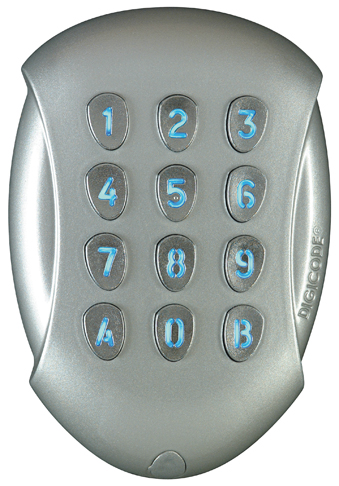
\includegraphics[width=.7\textwidth]{images/digicode}

\textit{Digicode}
\end{center}
\end{minipage}\hfill
\begin{minipage}[c]{.2\linewidth}
\begin{center}
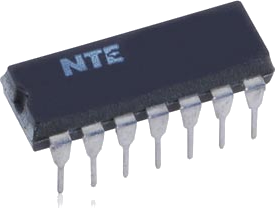
\includegraphics[width=.8\textwidth]{images/transistor_ttl_nand}

\textit{Transistor TTL (permettant de réaliser des opérations logiques) }
\end{center}
\end{minipage}\hfill
\begin{minipage}[c]{.2\linewidth}
\begin{center}
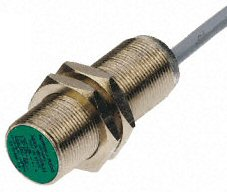
\includegraphics[width=.8\textwidth]{images/inductif}

\textit{Détecteur inductif}
\end{center}
\end{minipage}\hfill
\begin{minipage}[c]{.2\linewidth}
\begin{center}
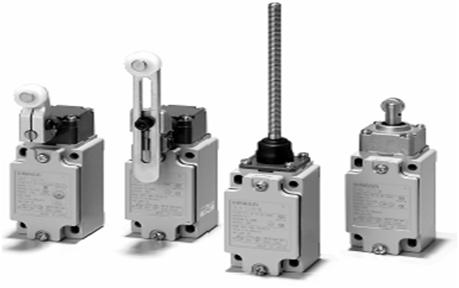
\includegraphics[width=\textwidth]{images/capteur_contact}

\textit{Détecteur à contact}
\end{center}
\end{minipage}

Un des objectifs de l'automaticien est de concevoir la partie commande qui traite les informations et élabore les ordres. Ce cours étudie le cas où les informations et les ordres élaborés sont des variables binaires.

\begin{savoir}
\textsc{Savoirs :}
\begin{itemize}
\item \textbf{Mod - C5.1 :} Modélisation des systèmes à événements discrets (fonctions logiques, tables de vérité).
\end{itemize}
\end{savoir}

%\newpage 

\setlength{\parskip}{0ex plus 0.2ex minus 0ex}
 \renewcommand{\contentsname}{}
 \renewcommand{\baselinestretch}{1}

\tableofcontents

 \renewcommand{\baselinestretch}{1.2}
\setlength{\parskip}{2ex plus 0.5ex minus 0.2ex}

% \vspace{1cm}
\textit{Ce document évolue. Merci de signaler toutes erreurs ou coquilles.}




\section{Numération, codage, transcodage}
\begin{rem}
On considère acquis les notions de systèmes de numérations décimaux, binaires et hexadécimaux ainsi que le passage d'une base à l'autre.

On considère aussi qu'il existe des notions sur la norme ASCII. 
\end{rem}

\subsection{Systèmes de codages utiles en technologie} 

\subsubsection{Code binaire naturel}
\begin{minipage}[c]{.65\linewidth}
Ce code pondéré correspond à donner un nombre selon sa valeur en système de numérotation binaire. 

C'est le seul code qui permet de réaliser des opérations. 

Inconvénient : il introduit des erreurs lors d'un changement de code. Pour passer de $(01)_2$ à $(10)_2$, donc de 1 à2, il faut modifier chaque digit et afficher (même brièvement) $(11)_2$ (soit 3) ou $(00)_2$ (soit 0). Cela peut provoquer des perturbations ou des erreurs. 
\end{minipage}\hfill
\begin{minipage}[c]{.32\linewidth}
\begin{center}
\begin{tabular}{|c|c|c|c||c|}
\hline
\multicolumn{4}{|c||}{Entrée} & Sortie \\ \hline \hline
0 & 0 & 0 & 0 & 0 \\ \hline 
0 & 0 & 0 & 1 & 1 \\ \hline
0 & 0 & 1 & 0 & 2 \\ \hline
0 & 0 & 1 & 1 & 3 \\ \hline
0 & 1 & 0 & 0 & 4 \\ \hline
0 & 1 & 0 & 1 & 5 \\ \hline
0 & 1 & 1 & 0 & 6 \\ \hline
0 & 1 & 1 & 1 & 7 \\ \hline
1 & 0 & 0 & 0 & 8 \\ \hline
1 & 0 & 0 & 1 & 9 \\ \hline
\end{tabular}
\vspace{.25cm}

\textit{Table de vérité du code binaire naturel}
\end{center} 
\end{minipage}

\vspace{.25cm}

\subsubsection{Code décimal codé binaire (DCB)}
C'est un code pondéré base sur le code binaire naturel mais qui est adapté à la représentation des nombres en base 10. En effet le code binaire pur n'associe pas des bits spécifiques aux unités, dizaines, centaines, ... La propriété du code DCB est d'associer 4 bits différents à chaque puissance de 10. Ainsi, 
$$
(1664)_{10} \quad \Longrightarrow \quad  (0001.0110.0110.0100)_{DCB}
$$

Ce code est utilisé pour les afficheurs 7 segments. Chaque afficheur reçoit le chiffre codé en binaire sur 4 bits. 

\begin{minipage}[c]{.6\linewidth}
Inconvénient : Cette représentation adaptée à la représentation binaire des nombres décimaux utilise un nombre de bits supérieur à celui du binaire naturel, et donc une place plus important en mémoire de l'ordinateur. 
\end{minipage} \hfill
\begin{minipage}[c]{.25\linewidth}
\begin{center}
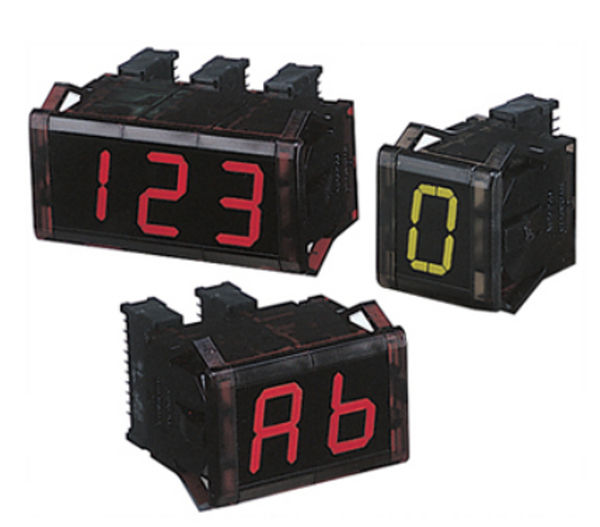
\includegraphics[width=.8\textwidth]{images/fig_03}
\end{center}
\end{minipage}

\begin{rem}
On peut réaliser la même typologie pour le code hexadécimal. Notons ce codage HCB. Ainsi,
$$
(0C3F)_{16} \quad \Longrightarrow \quad (0000.1100.0011.1111)_{HCB}
$$
\end{rem}

\subsubsection{Code  binaire réfléchi ou code Gray}
\begin{minipage}[c]{.55\linewidth}
Ce code non pondéré est un arrangement du système binaire. Le passage d'un nombre à l'autre se fait en changeant l'état d'un seul bit. Il est très utilisé pour décrire des automatismes (un changement d'état d'un composant correspond à un bit qui change), en particulier dans les codeurs de position absolue. 

Avantage : il apporte une garantie d'interprétation avec une erreur maximale d'incrémentation. 

\begin{center}
\begin{tabular}{cc}
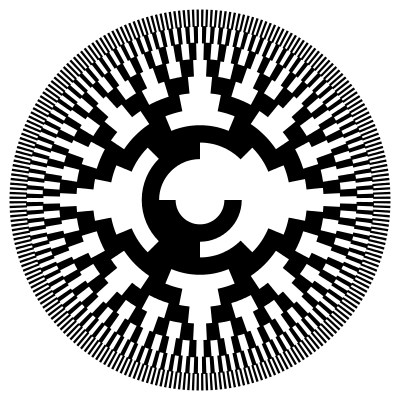
\includegraphics[height=4cm]{images/DisqueGray} &
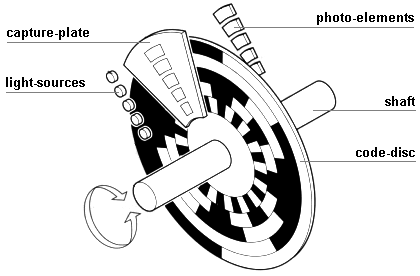
\includegraphics[height=3.5cm]{images/CodeurGray} \\
\textit{Disque codage Gray} & 
\textit{Disque codage Gray} \\
\end{tabular}



\end{center}

Pour obtenir le code Gray, il faut faire toutes les $2^1$, $2^2$, $2^3$ ... lignes, une symétrie en commençant par le bit de droite et changer la valeur du bit de gauche. 

\end{minipage}\hfill
\begin{minipage}[c]{.4\linewidth}
\begin{center}
\begin{tabular}{|c|cccc|cccc|}
\hline
Décimal & \multicolumn{4}{c|}{Binaire pur} &\multicolumn{4}{c|}{Binaire réfléchi} \\
\hline
\hline
0 & 0 & 0 & 0 & 0 & 0 & 0 & 0 & 0 \\ \hline
1 & 0 & 0 & 0 & 1 & 0 & 0 & 0 & 1 \\ \hline\hline
2 & 0 & 0 & 1 & 0 & 0 & 0 & 1 & 1 \\ \hline
3 & 0 & 0 & 1 & 1 & 0 & 0 & 1 & 0 \\ \hline\hline
4 & 0 & 1 & 0 & 0 & 0 & 1 & 1 & 0 \\ \hline
5 & 0 & 1 & 0 & 1 & 0 & 1 & 1 & 1 \\ \hline
6 & 0 & 1 & 1 & 0 & 0 & 1 & 0 & 1 \\ \hline
7 & 0 & 1 & 1 & 1 & 0 & 1 & 0 & 0 \\ \hline\hline
8 & 1 & 0 & 0 & 0 & 1 & 1 & 0 & 0 \\ \hline
9 & 1 & 0 & 0 & 1 & 1 & 1 & 0 & 0 \\ \hline
10 & 1 & 0 & 1 & 0 & 1 & 1 & 1 & 1 \\ \hline
11 & 1 & 0 & 1 & 1 & 1 & 1 & 1 & 1 \\ \hline
12 & 1 & 1 & 0 & 0 & 1 & 0 & 1 & 0 \\ \hline
13 & 1 & 1 & 0 & 1 & 1 & 0 & 1 & 0 \\ \hline
14 & 1 & 1 & 1 & 0 & 1 & 0 & 0 & 1 \\ \hline
15 & 1 & 1 & 1 & 1 & 1 & 0 & 0 & 0 \\ \hline
\end{tabular}
\end{center}
\end{minipage}
%\begin{exemple}
%Écrire en code Gray le nombre 56.
%\end{exemple}

\subsection{Les codeurs optiques}
\subsubsection{Le codeur incrémental}
\begin{minipage}[c]{.75\linewidth}
Un codeur incrémental est constitué d'un disque généralement muni de deux pistes ainsi que de trois couples de DEL -- récepteurs. Une des deux pistes est percée d'une seule fente. Le détecteur noté $Z$ permet de détecter le passage de cette fente. La seconde piste est composée de $n$ fentes. Les deux autres DEL ($A$ et $B$) détectent le passage des fentes sur cette piste. 

Dans certains cas, les impulsions peuvent être mesurées par des capteurs à effets Hall. 

Ces codeurs permettent de réaliser une mesure incrémentale. Il faut donc fixer une référence (POM -- Prise d'Origine Machine) pour connaitre la position absolue.

Ces codeurs sont utilisés pour mesurer les déplacements des axes sur les machines outils. On en retrouve aussi sur l'axe asservi Emericc ou encore sur le Tribar.
\end{minipage}\hfill
\begin{minipage}[c]{.2\linewidth}
\begin{center}
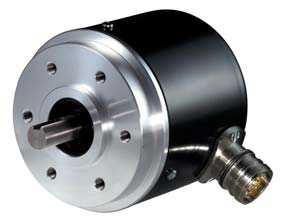
\includegraphics[width=.95\textwidth]{images/CodeurIncremental}
\end{center}
\end{minipage}

\begin{exemple}
\begin{minipage}[c]{.75\linewidth}

La résolution d'un codeur incrémental peut varier de 1 000 à 25 000 impulsions par tour pour des fréquences de rotation allant jusqu'à 10 000 tr/min.
\begin{enumerate}
\item Donner la résolution en degrés du codeur. 
\item Quelle doit être la fréquence minimale du système d'acquisition afin de pouvoir gérer les informations provenant du codeur ?
\item Réaliser le chronogramme des sorties des voies $A$ et $B$ en faisant l'hypothèse que les DEL $A$ et $B$ sont <<décalées>> d'un quart de période.
\item Expliquer en quoi l'existence des deux LED permet de détecter le sens de rotation du disque. 
\end{enumerate}
\end{minipage}\hfill
\begin{minipage}[c]{.2\linewidth}
\begin{center}
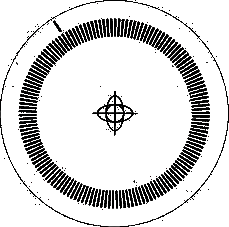
\includegraphics[width=.95\textwidth]{images/DisqueIncremental}
\end{center}
\end{minipage}

\begin{minipage}[c]{.45\linewidth}
\begin{center}
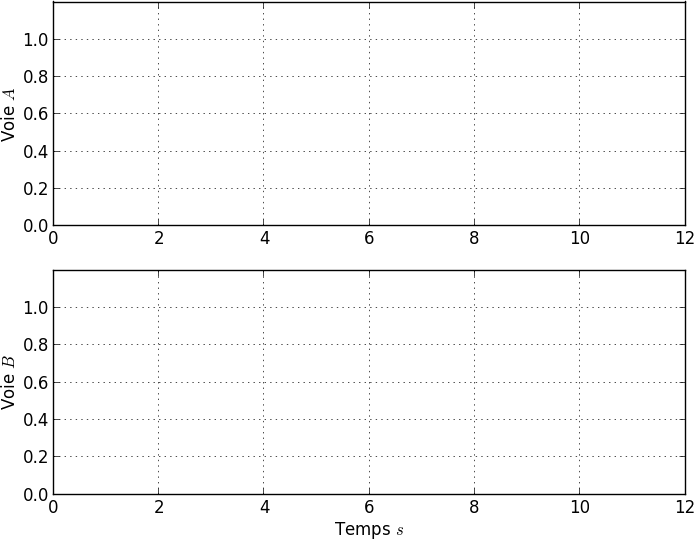
\includegraphics[width=\textwidth]{images/ChronogrammeIncremental}
\end{center}
\end{minipage} \hfill
\begin{minipage}[c]{.45\linewidth}
\begin{center}
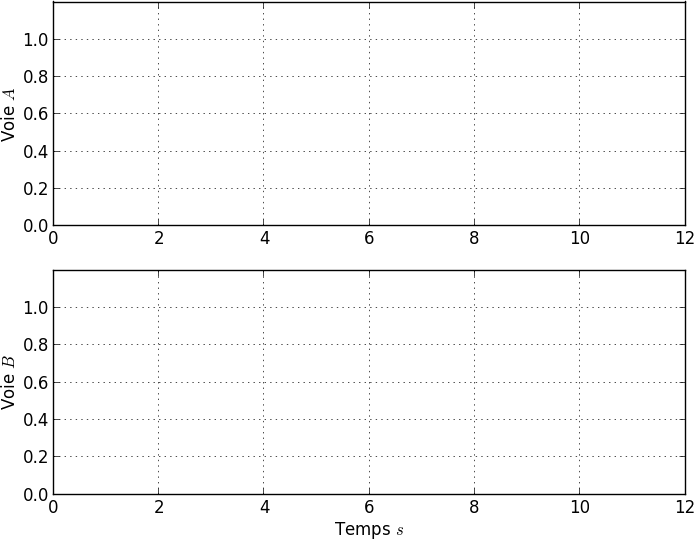
\includegraphics[width=\textwidth]{images/ChronogrammeIncremental}
\end{center}
\end{minipage}
\end{exemple}



\subsubsection{Le codeur absolu}

Un codeur absolu permet de déterminer la position angulaire réel d'un système. Il est constitué de $N$ pistes avec des fentes qui sont agencées selon le codage Gray. Une <<rampe>> de $N$ couples de DEL -- récepteurs permettent de détecter, à un instant donné une combinaison de bits correspondant à la position du disque. 

\begin{exemple}
\begin{enumerate}
\item Combien de pistes faut-il pour coder $360 \textdegree$ avec une précision de $0,1 \textdegree$. 
\item Combien faudrait-il de fentes avec codeur incrémental ? 
\item Pour un codeur avec 3 pistes, teinter les différentes zones dans le cas d'un codage Gray puis dans le cas d'un codeur naturel.
\item Conclure sur l'intérêt du code Gray lorsque les DEL sont décalées. 
\end{enumerate}

\begin{minipage}[c]{.45\linewidth}
\begin{center}
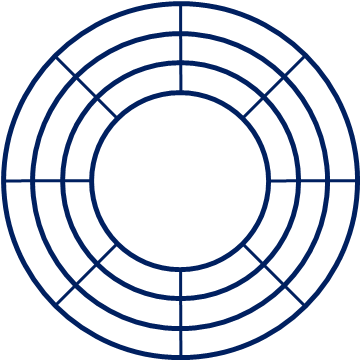
\includegraphics[width=.8\textwidth]{images/DisqueAbsolu}

\textit{Codage binaire naturel}
\end{center}
\end{minipage} \hfill
\begin{minipage}[c]{.45\linewidth}
\begin{center}
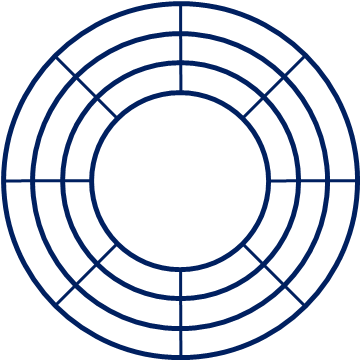
\includegraphics[width=.8\textwidth]{images/DisqueAbsolu}

\textit{Codage binaire réfléchi}
\end{center}
\end{minipage}


\end{exemple}

\section{Systèmes combinatoires}
%
%\begin{exemple}
%Support : éclairage d'un escalier
%
%On souhaite éclairer un escalier par 4 lampes qui s'allument automatiquement lorsque l'on monte ou descend l'escalier. Pour l'esthétisme, on désire que les lampes s'allument puis s'éteignent successivement lorsqu'une présence est détectée. On utilise 3 détecteurs de présence notés $a$, $b$, et $c$. L'objectif est de déterminer les équations logiques liant l'état des lampes à l'état des détecteurs de présence. Chaque capteur détecte une présence. Chaque capteur détecte une présence dans la zone indiquée. Il faut toujours 2 lampes allumées sauf aux marches extrêmes. 
%\end{exemple}
%
%
%\begin{center}
%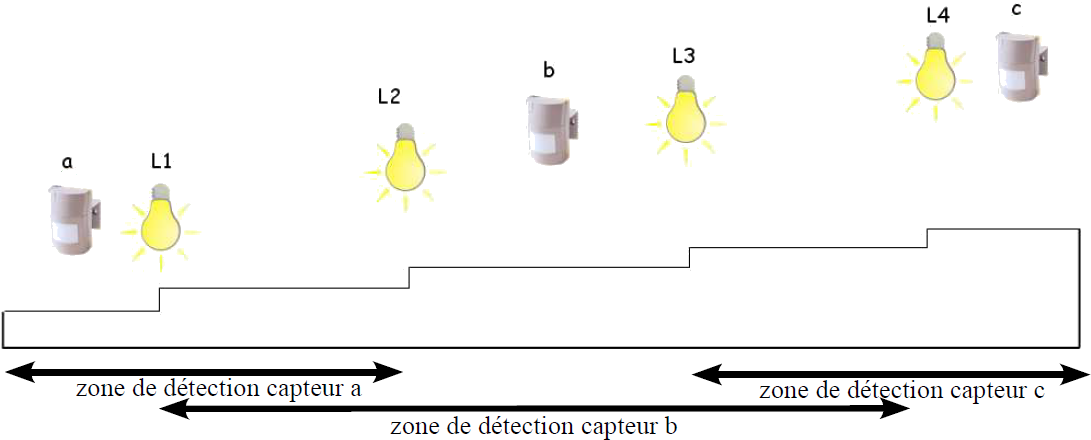
\includegraphics[width=.9\textwidth]{images/fig_06}
%\end{center}


\subsection{Définitions}
\subsubsection{Variables binaires}
De nombreux composants utilisés en automatisme ne peuvent normalement prendre que deux états différents : lampe allumée ou éteinte, bouton-poussoir actionné ou relâché, moteur tournant ou à l'arrêt, vérin pneumatique sorti ou rentré. 


A chacun de ces composants, on peut associer une variable binaire (ou logique, Tout Ou Rien) qui ne peut prendre que deux valeurs notées 0 ou 1 (vrai ou faux, oui ou non). 

\begin{defi}
Une variable $a$ est binaire si et seulement si elle peut prendre, à chaque instant, qu'une seule valeur parmi un ensemble de 2 valeurs possibles. 
\end{defi}

\begin{exemple}
\textit{Lister les variables binaires pour un codeur incrémental avec une résolution de 0,1 degrés et pour un codeur absolu de même résolution.}
\end{exemple}


\begin{rem}
\begin{minipage}[c]{.6\linewidth}
Le comportement tout ou rien (TOR) ne correspond qu'au comportement normalement prévu en régime stabilisé et en l'absence de tout dysfonctionnement. 

L'association d'une variable binaire à un composant ne peut pas rendre compte des états transitoires apparaissent entre deux états stables. C'est donc une simplification du comportement réel.
\end{minipage}\hfill
\begin{minipage}[c]{.35\linewidth}
\begin{center}
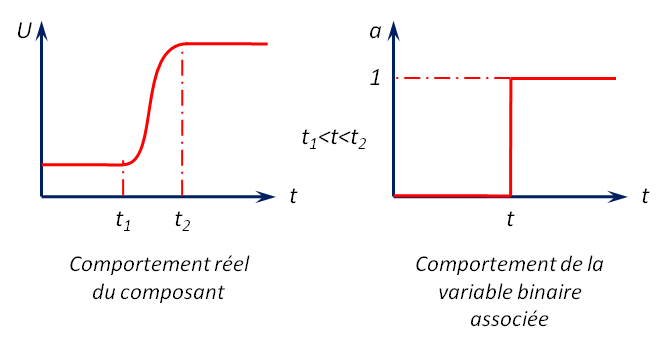
\includegraphics[width=\textwidth]{images/fig_07_2}
\end{center}
\end{minipage}
\end{rem}



\subsubsection{Système binaire}

\begin{defi}
Un système est dit binaire ou logique si les variables d'entrée et de sortie sont binaires. 
\end{defi}

\subsubsection{Systèmes combinatoire et séquentiel}
\begin{defi}
Un système logique combinatoire est un système binaire pour lequel à un état des variables d'entrée $E_i$ correspond un unique état des variables de sortie $S_j$. (La réciproque n'est pas vraie.)
\end{defi}

\begin{center}
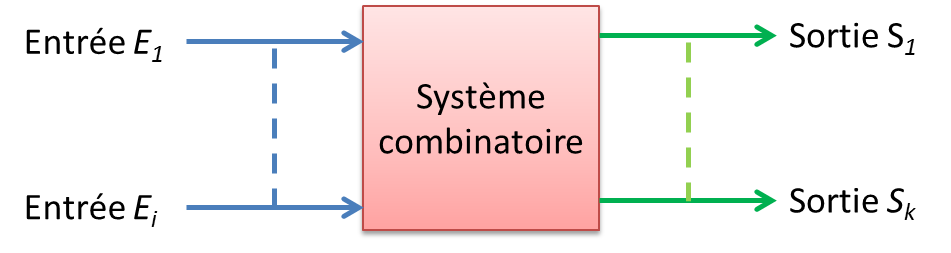
\includegraphics[width=.6\textwidth]{images/fig_08}
\end{center}

\begin{defi}
Un système logique est dit séquentiel si les sorties $S_j$ ne dépendent pas uniquement des $E_i$.
\end{defi}

\begin{exemple}
\begin{center}
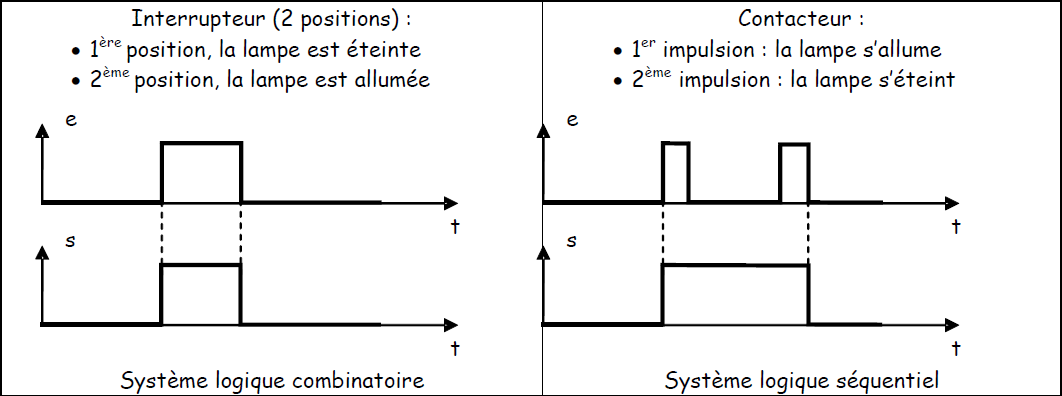
\includegraphics[width=.9\textwidth]{images/fig_09}
\end{center}

\end{exemple}


\subsection{Algèbre de Boole}

La fonction logique qui caractérise le système est indépendante du temps. Pour traiter de tels systèmes, on utilise l'algèbre de Boole. 

\subsubsection{Définition}
C'est un algèbre de propositions logiques mise au point par un mathématicien anglais, Georges Boole (1815 -- 1864).

\begin{defi}
Un ensemble $E$ a une structure d'algèbre Boole si on a défini dans cet ensemble :
\begin{itemize}
\item une relation d'équivalence notée $=$;
\item deux lois de composition interne $+$ (addition booléenne) et $\cdot$ (multiplication booléenne);
\item une loi appelée complémentation ($\overline{a}$ complément de $a$).
\end{itemize}
\end{defi}

Une algèbre binaire est une algèbre de Boole dont les éléments $B$ ne peuvent prendre que deux valeurs notées 0 ou 1 : $B=\{0,1 \}$. 

\begin{exemple}
Fonction OUI.

\begin{center}
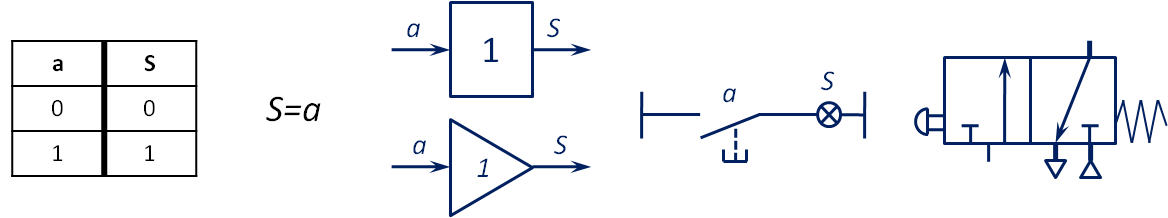
\includegraphics[width=.9\textwidth]{images/oui}
\end{center}
\end{exemple}


\subsubsection{Fonction NON -- appelée complément}
\begin{defi}
\textbf{Fonction NON -- appelée complément}

\begin{minipage}[c]{.45\linewidth}
\begin{eqnarray*}
B &\longmapsto& B\\
a &\longmapsto& \overline{a}
\end{eqnarray*}
Il faut lire $\overline{a}$ : NON a.
\end{minipage} \hfill
\begin{minipage}[c]{.45\linewidth}
\begin{center}
\begin{tabular}{|c||c|}
\hline
$a$ & $\overline{a}$ \\
\hline
0 & 1 \\
\hline
1 & 0 \\
\hline
\end{tabular}
\end{center}
\end{minipage}
\end{defi}

\begin{exemple}
Fonction NON.


\begin{center}
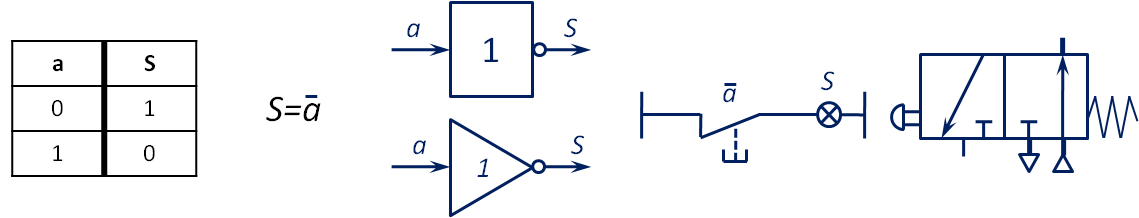
\includegraphics[width=.9\textwidth]{images/NON}
\end{center}

\end{exemple}


\subsubsection{Fonction ET -- Produit booléen}

\begin{defi}
\textbf{Fonction ET -- Produit booléen}

\begin{minipage}[c]{.45\linewidth}
\begin{eqnarray*}
B \times B &\longmapsto& B\\
(a,b) &\longmapsto& a \cdot b
\end{eqnarray*}
Il faut lire $a$ ET $b$. 
\end{minipage} \hfill
\begin{minipage}[c]{.45\linewidth}
\begin{center}
\begin{tabular}{|c|c||c|}
\hline
$a$ & $b$ & $a\cdot b$ \\
\hline
0 & 0 & 0 \\ \hline
0 & 1 & 0 \\ \hline
1 & 0 & 0 \\ \hline
1 & 1 & 1 \\ \hline
\end{tabular}
\end{center}
\end{minipage}
\end{defi}

\begin{exemple}

\begin{center}
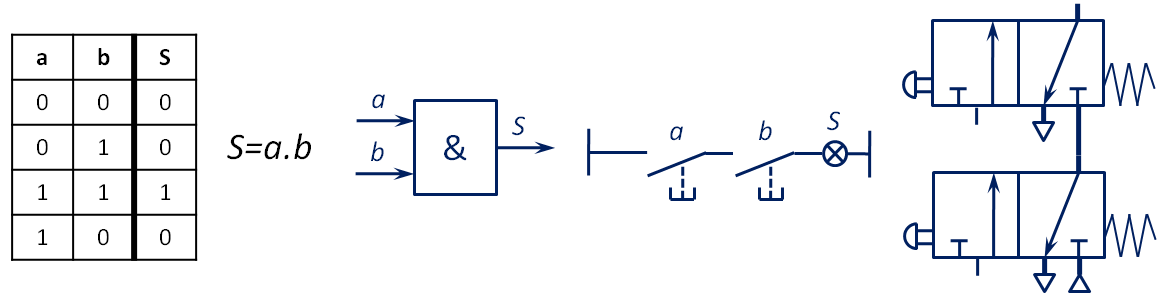
\includegraphics[width=.9\textwidth]{images/ET}
\end{center}

\end{exemple}


\subsubsection{Fonction OU -- Somme booléenne}


\begin{defi}
\textbf{Fonction OU -- Somme booléenne}

\begin{minipage}[c]{.45\linewidth}
\begin{eqnarray*}
B \times B &\longmapsto& B\\
(a,b) &\longmapsto& a + b
\end{eqnarray*}
Il faut lire $a$ OU $b$. 
\end{minipage} \hfill
\begin{minipage}[c]{.45\linewidth}
\begin{center}
\begin{tabular}{|c|c||c|}
\hline
$a$ & $b$ & $a+ b$ \\
\hline
0 & 0 & 0 \\ \hline
0 & 1 & 1 \\ \hline
1 & 0 & 1 \\ \hline
1 & 1 & 1 \\ \hline
\end{tabular}
\end{center}
\end{minipage}
\end{defi}

\begin{exemple}
Fonction OU.


\begin{center}
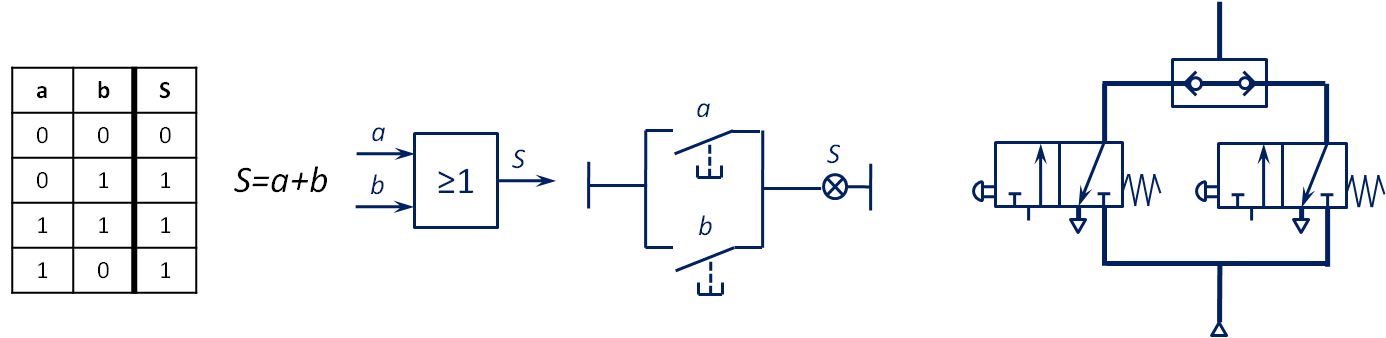
\includegraphics[width=.9\textwidth]{images/OU}
\end{center}
\end{exemple}

\subsubsection{Propriétés des opérateurs de base de l'algèbre de Boole}

\begin{prop}
\textbf{Commutativité}

\begin{minipage}[c]{.45\linewidth}
$$ a+b = b+a$$
\end{minipage}\hfill
\begin{minipage}[c]{.45\linewidth}
$$ a\cdot b = b\cdot a$$
\end{minipage}

\textbf{Distributivité}

\begin{minipage}[c]{.45\linewidth}
$$ a\cdot (b+c) = a\cdot b+a \cdot c$$
\end{minipage}\hfill
\begin{minipage}[c]{.45\linewidth}
$$ a+(b\cdot c) = (a+b) \cdot (a+c)$$
\end{minipage}

\textbf{Associativité}

\begin{minipage}[c]{.45\linewidth}
$$ a + (b+c) = (a+b)+c = a+b+c$$
\end{minipage}\hfill
\begin{minipage}[c]{.45\linewidth}
$$ a \cdot (b\cdot c) = (a\cdot b)\cdot c = a \cdot b\cdot c$$
\end{minipage}

\textbf{Élément neutre}

\begin{minipage}[c]{.45\linewidth}
$$ a + 0 = a$$
\end{minipage}\hfill
\begin{minipage}[c]{.45\linewidth}
$$ a\cdot 1 = a$$
\end{minipage}

\textbf{Élément absorbant}

\begin{minipage}[c]{.45\linewidth}
$$ a + 1 = 1$$
\end{minipage}\hfill
\begin{minipage}[c]{.45\linewidth}
$$ a\cdot 0 = 0$$
\end{minipage}

\textbf{Complémentarité}

\begin{minipage}[c]{.45\linewidth}
$$ a + \overline{a} = 1$$
\end{minipage}\hfill
\begin{minipage}[c]{.45\linewidth}
$$ a\cdot \overline{a} = 0$$
\end{minipage}

Par ailleurs $\overline{\overline{a}}=a$.

\textbf{Idem potence}

\begin{minipage}[c]{.45\linewidth}
$$ a + a = a$$
\end{minipage}\hfill
\begin{minipage}[c]{.45\linewidth}
$$ a\cdot a = a$$
\end{minipage}

\textbf{Identités remarquables}

Absorption : 
$$ a + a\cdot b = a$$

Inclusion :
$$
a+\overline{a}\cdot b = a+b
$$
\end{prop}

\subsubsection{Théorème de Morgan}
\begin{theo}
$$
\overline{\sum\limits_{i=1}^{n} a_i} = \prod\limits_{i=1}^n \overline{a_i}
\quad
\overline{\prod\limits_{i=1}^{n} a_i} = \sum\limits_{i=1}^n \overline{a_i}
$$
\end{theo}

\begin{exemple}
Déterminer les expressions complémentaires $\overline{P}$ et $\overline{Q}$ des expressions suivantes : 
$P = x\cdot y \cdot (z + \overline{t})$ et $Q=\overline{x}\cdot\overline{y} + y + x\cdot t$.
\end{exemple}

\section{Fonctions logiques}

Un système combinatoire est décrit par une fonction logique qui permet de définir de manière unique la sortie pour une combinaison des entrées. 

\subsection{Table de vérité}
La table de vérité d'une fonction logique est une écriture systématique qui consiste à décrire toutes les combinaison des variables et à y associer les valeurs correspondantes de la fonction. 

\begin{exemple}


Compléter la table de vérité suivante et vérifier les théorèmes de De Morgan pour deux variables.
\begin{center}
\begin{tabular}[c]{|c|c||c|c|c|c|}
\hline
$a$ & $b$ & $\overline{a\cdot b}$ & $\overline{a} + \overline{b}$ & $\overline{a+b}$ & $\overline{a}\cdot\overline{b}$ \\
\hline \hline 
0 & 0 & & & & \\ \hline
0 & 1 & & & & \\ \hline
1 & 1 & & & & \\ \hline
1 & 1 & & & & \\ \hline
\end{tabular}
\end{center}

\end{exemple}

\begin{exemple}
Soit 4 lampes $L_1$, $L_2$, $L_3$, $L_4$ permettant d'éclairer un escalier. L'allumage de ces 3 lampes est régit par 3 détecteurs de présences $a$, $b$ et $c$. La table de vérité est la suivante :

\begin{minipage}[c]{.4\linewidth}
\begin{center}
\begin{tabular}[c]{|c|c|c||c|c|c|c|}
\hline 
$a$ & $b$ & $c$ & $L_1$ & $L_2$ & $L_3$ & $L_4$ \\
\hline \hline
0 & 0 & 0 & 0 & 0 & 0 & 0 \\ \hline
0 & 0 & 1 & 0 & 0 & 0 & 1 \\ \hline
0 & 1 & 1 & 0 & 0 & 1 & 1 \\ \hline
0 & 1 & 0 & 0 & 1 & 1 & 0 \\ \hline
1 & 1 & 0 & 1 & 1 & 0 & 0 \\ \hline
1 & 1 & 1 & 1 & 1 & 1 & 1 \\ \hline
1 & 0 & 1 & 1 & 0 & 0 & 1 \\ \hline
1 & 0 & 0 & 1 & 0 & 0 & 0 \\ \hline 
\end{tabular}
\end{center}
\end{minipage}
\begin{minipage}[c]{.55\linewidth}
\begin{center}
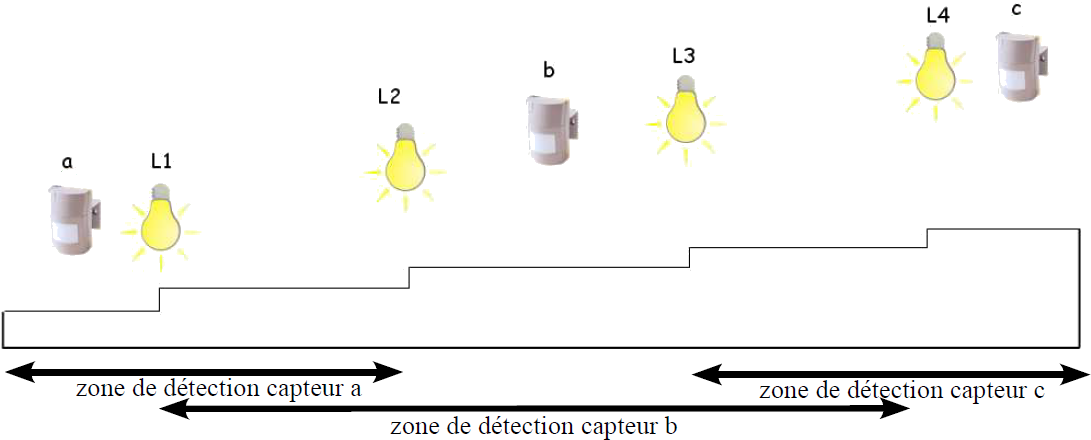
\includegraphics[width=\textwidth]{images/fig_06}
\end{center}
\end{minipage}

Donner l'expression de $L_1$, $L_2$, $L_3$, $L_4$.
\end{exemple}

Il est possible à l'aide de la table de vérité de définir une équation donnant les variables de sortie en fonction des variables d'entrée. Il existe 2 modes d'écriture particuliers : 
\begin{itemize}
\item somme canonique (somme de produit) : $S=a\cdot b + c\cdot d$;
\item produit canonique (produit de sommes) : $S=(a+b) \cdot (c+d)$.
\end{itemize}

\begin{methode}
\textbf{Détermination de la somme canonique}

Pour chaque ligne où la sortie vaut 1, déterminer la combinaison d'entrées correspondante à l'aide de l'opérateur ET puis sommer ces combinaisons. 
\end{methode}


\begin{exemple}
Donner l'expression sous forme canonique de $L_1$ et $L_2$ à partir de la table de vérité précédente. 
\end{exemple}

\begin{rem}
On utilise la forme de sommes canoniques si le nombre de 1 est inférieur au nombre de 0. Il est souvent nécessaire de simplifier ces équations pour réaliser technologiquement ces fonctions (voir plus loin).
\end{rem}

\begin{methode}
\textbf{Détermination du produit canonique}

Déterminer l'expression de $\overline{S}$ ce qui revient à :
Déterminer la combinaison d'entrées pour chaque ligne où la sortie vaut 0, les sommer, puis passez au complémentaire en utilisant les théorèmes de De Morgan. 
\end{methode}

\begin{exemple}
Donner l'expression sous forme de produit canonique de $L_1$ et $L_2$.
\end{exemple}

\begin{rem}
Cette méthode est utile lorsque la sortie comporte peu de 0 et beaucoup de 1 ou lorsque l'on recherche la fonction complémentaire. 
\end{rem}

\section{Simplification des fonctions logiques}
La simplification des expressions logiques est destinée à économiser le matériel nécessaire à la réalisation (utilisation d'un composant réalisant plusieurs fonctions identiques) ou diminuer l'importance des équations programmées.

\subsection{Cellules universelles}
\begin{defi}

Une cellule (ou fonction) est dite "universelle" si elle permet de réaliser les fonctions ET, OU, NON. Il est alors possible de réaliser toutes les fonctions logiques à l'aide de cette seule cellule. 
\end{defi}

\begin{exemple}
Les cellules NAND (non et -- $a NAND b = \overline{a\cdot b}$) et NOR (non ou -- $a NOR b = \overline{a + b}$) sont des cellules universelles. 

Réalisation de la fonction NON : $ NON(a) = \overline{a} = \overline{a\cdot a}$. Besoin d'une seule cellule NAND. 
 
Réalisation de la fonction ET : $ a ET b = a\cdot b= \overline{\overline{a\cdot b}} $. Besoin de deux cellules NAND en cascade. 

Réalisation de la fonction OU : $ a OU b = a+ b= \overline{\overline{a+b}}= \overline{\overline{a}\cdot\overline{b}} $. Besoin de trois cellules NAND en cascade. 

De même, la cellule NOR est universelle.
\end{exemple}

\begin{exemple}
Écrire l'expression logique suivante uniquement avec des opérateurs NAND puis indiquer le nombre minimal d'opérateurs utilisés.
$$
F=c\cdot (\overline{a}+\overline{b})
$$
\end{exemple}

\subsection{Simplification algébrique d'une fonction}
Il s'agit d'utiliser les propriétés, théorèmes et identités remarquables de l'algèbre de Boole afin de simplifier une équation. Cette méthode n'est pas forcément simple à utiliser et demande beaucoup d'intuition.

\begin{exemple}
$$F(a,b,c) = \overline{a}\cdot \overline{b} \cdot c + a \cdot \overline{b} \cdot c + \overline{a}\cdot b \cdot c = \overline{a}\cdot c \cdot (\overline{b}+b) + a\cdot \overline{b}\cdot c = \overline{a}\cdot c + a\cdot \overline{b}\cdot c = c(\overline{a}+a\cdot \overline{b}) = c\left(\overline{a}(1+\overline{b}) + a \cdot \overline{b}\right) = c\cdot (\overline{a}+\overline{b})$$
\end{exemple}

\begin{exemple}
Simplifier par cette méthode l'expression des lampes $L_1$ et $L_2$. 
\end{exemple}




\section{Représentation des fonctions logiques}
Dans un système combinatoire : 
\begin{itemize}
\item les variables d'entrée sont des informations qui décrivent à un moment donnée l'état de certaines parties (position d'un chariot, d'un outil, ...)
\item les variables de sortie permettent de décrire l'état dans lequel doivent se retrouver les organes récepteurs. 
\end{itemize}

Une fois l'expression logique obtenue et simplifiée, il est possible d'exprimer graphiquement le comportement du système combinatoire. On utilise pour cela en général le logigramme ou le schéma électrique. On peut également utiliser un schéma pneumatique ou électronique.


%Un logigramme est une représentation logique 


\begin{center}
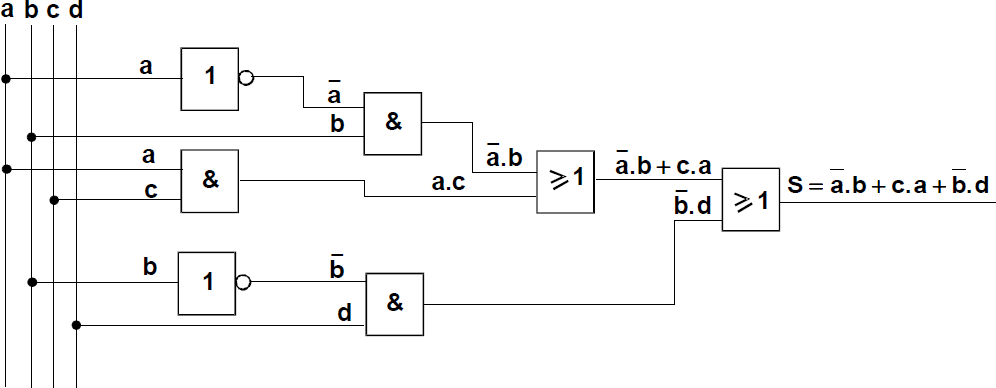
\includegraphics[width=.6\textwidth]{images/fig_17}
\end{center}


\subsection{Logigrammes pour un codeur incrémental}
\begin{exemple}
\begin{enumerate}
\item Réaliser le logigramme illustrant le comptage et le décomptage des impulsions provenant d'un codeur incrémental.
\item Réaliser le logigramme illustrant le comptage et le décomptage des impulsions provenant d'un codeur incrémental en multipliant par 4 sa résolution.
\end{enumerate}

\begin{rem}
On appelera front montant de $a$ et notera $\uparrow a$  le passage de la variable $a$ de l'état 0 à l'état 1.
\end{rem}

\end{exemple}

\begin{thebibliography}{2}
\bibitem{dv}{Supports de cours de David Violeau, Lycée Saint-Louis, Paris.}
\bibitem{fm}{Supports de cours de Florestan Mathurin, Lycée Bellevue, Toulouse.}
%\bibitem{jpp}{Supports de cours de Jean-Pierre Pupier, Lycée Rouvière, Toulon}

\end{thebibliography}

\end{document}\end{document}


